\documentclass[12pt,a4paper,titlepage,ngerman,pdftex]{report}
\usepackage[utf8]{inputenc}
\usepackage[german]{babel}
\usepackage[T1]{fontenc}
\usepackage{amsmath}
\usepackage{amsfonts}
\usepackage{amssymb}
\usepackage{graphicx}
\usepackage{acronym}
\usepackage{setspace}
\usepackage{geometry}
\usepackage{caption}
\usepackage{subcaption}
\usepackage{hyperref}
\usepackage{listings}
\usepackage{textcomp}
\usepackage{footnote}
\geometry{a4paper, top=25mm, left=25mm, right=25mm, bottom=25mm,
    headsep=10mm, footskip=12mm}
\usepackage{xcolor}

\definecolor{mygreen}{rgb}{0,0.6,0}
\definecolor{mygray}{rgb}{0.5,0.5,0.5}
\definecolor{mymauve}{rgb}{0.58,0,0.82}
\definecolor{backcolour}{rgb}{0.827, 0.827, 0.827}
\definecolor{dkblue}{rgb}{0,0,.6}
\definecolor{dkyellow}{cmyk}{0,0,.8,.3}

\lstset{
    language        = php,
    basicstyle      = \small\ttfamily,
    keywordstyle    = \color{dkblue},
    stringstyle     = \color{red},
    identifierstyle = \color{mygreen},
    commentstyle    = \color{gray},
    emph            =[1]{php},
    emphstyle       =[1]\color{black},
    emph            =[2]{if,and,or,else},
    emphstyle       =[2]\color{dkyellow}}

\lstset{ %
    backgroundcolor=\color{backcolour},   % choose the background color
    basicstyle=\footnotesize,        % size of fonts used for the code
    breaklines=true,                 % automatic line breaking only at whitespace
    captionpos=b,                    % sets the caption-position to bottom
    commentstyle=\color{mygreen},    % comment style
    escapeinside={\%*}{*)},          % if you want to add LaTeX within your code
    keywordstyle=\color{blue},       % keyword style
    stringstyle=\color{mymauve},     % string literal stylebreakatwhitespace=false,
    keepspaces=true,
    numbers=left,
    numbersep=5pt,
    showspaces=false,
    showstringspaces=true,
    showtabs=false,
    tabsize=2
}

\begin{document}
%%%%%%%%%%%%%%%%%%%%%%%%%%%%%%%%%%%%%%%%%%%%%%%
%%%%%%%%%%%%%%%%%    TITLE    %%%%%%%%%%%%%%%%%
%%%%%%%%%%%%%%%%%%%%%%%%%%%%%%%%%%%%%%%%%%%%%%%
    \begin{titlepage}
        \centering
        %\includegraphics[width=0.15\textwidth]{pic/picsim_logo_full.png}\par\vspace{1cm}
        {\scshape\LARGE Duale Hochschule Baden-Württemberg \par}
        \vspace{1cm}
        {\scshape\Large Advanced Software Engineering 2 \\--\\ Dokumentation\par}
        \vspace{1.5cm}
        {\huge\bfseries PIC-Simulator\par}
        \vspace{2cm}
        {\Large\itshape David Eymann, Tom Wagner\par}
        \vfill
        Dozent\par
        Daniel \textsc{Lindner}

        \vfill

% Bottom of the page
        {\large \today\par}
    \end{titlepage}

%%%%%%%%%%%%%%%%%%%%%%%%%%%%%%%%%%%%%%%%%%%%%%%
%%%%%%%%%%%%%%%%%  LISTINGS  %%%%%%%%%%%%%%%%%
%%%%%%%%%%%%%%%%%%%%%%%%%%%%%%%%%%%%%%%%%%%%%%%
    \pagenumbering{Roman}
    \tableofcontents
    \listoffigures
    \lstlistoflistings

    \onehalfspacing
    \pagenumbering{arabic}

    \chapter{Projektbeschreibung}\label{ch:projektbeschreibung}

    Als Basis für diese Arbeit dient ein PIC-Simulator, PIC steht hierbei für ein Mikrocontroller von Microchip Technology\footnote{\url{https://en.wikipedia.org/wiki/Microchip_Technology}}.
    Der Simulator ist in C\# geschrieben und mit Windows Forms Erhält er seine Grafische Oberfläche.
    \textbf{Das für diese Abgabe relevante Repository befindet sich unter:} \\ \url{https://github.com/tomwgnr/ASE-PIC_Simulator}\\

    
    

    \section{Einrichtung}\label{sec:einrichtung}

    \chapter{Entwicklung}\label{ch:entwicklung}
    \section{Clean Architecture}\label{sec:cleanarchitecture}

    Eine Clean Architecture ist wichtig, um langlebige Software zu entwickeln. Hierbei wird der Code in Schichten unterteilt, welche sich durch deren Lebensdauer unterscheiden. Die innerste Schicht ist dabei der Kern der Applikation, also der Teil des Codes der nicht verändert werden muss.
    Je weiter außen die Schicht ist, desto kurzlebiger ist der Code sodass ganz außen die Plugins stehen die nach einer gewissen Zeit outdated sind und ausgetauscht werden müssen um die Software Aktuell zu halten. 
    Damit diese Austauschbarkeit möglich ist, dürfen die inneren Schichten nichts von den äußeren wissen, es darf also keine Abhängigkeiten von innen nach außen geben.
    \\

    Für dieses Projekt haben wir und für drei Schichten entschieden: Eine Domain Schicht, welche den Kern des PIC- Simulators beschreibt, eine Application Schicht, in dem die Use Cases definiert sind, und einer Plugin Schicht, welche die GUI beschreibt.

    \subsection{Domain}
    In der Domain Schicht befinden sich die Elemente des PIC- Simulators, welche sich nicht ändern werden. Dazu gehören zu einen die einzelnen Commands und der Speicher des Simulators. Dabei handelt es sich konkret um die 'Command'- Klasse mit den jeweiligen Unterklassen, die 'Memory'- Klasse, 
    welche alle Speicherzugriffe bearbeitet sowie die einzelnen Register Klassen, welche den Aufbau des Speichers definieren. Diese Klassen haben alle keinerlei Abhängigkeiten nach außen und werden somit nicht von Veränderungen an den anderen Schichten beeinflusst.

    \subsection{Application}
    In der Application Schicht sind die einzelnen Use Cases beziehungsweise die Funktionalitäten des Projekts zu finden. Teil dieser Schicht ist die 'Simulator'- Klasse, welche den generellen Programmablauf steuert. Von ihr werden auch die anderen Klassen der Application Schicht aufgerufen.
    Es gibt den Decoder, welcher den eingelesenen Operationcode ananlysiert und den entsprechenden Handler, also den entsprechenden Command in der Domain Schicht aufruft. Außerdem befinden sich hier die 'InteruptChecker'- und 'FlankenChecker'-Klassen, welche Interrupts im PIC Simulieren, bzw abarbeiten.
    Diese Klassen haben lediglich Abhängigkeiten zu der 'Memory'-Klasse also der Domain. 

    \subsection{Plugin}
    In der Plugin Schicht befindet sich die 'Form1'-Klasse. Darin befindet sich die Konkrete implementierung der GUI, welche auf Windows Forms basiert. Der gesamte Code ist stark Framework abhängig, weshalb er in der äußersten Schicht plaziert ist.
    Soll statt Forms eine andere Bibliothek/ Framework verwendet werden, kann dies ohne großen Aufwand ausgetauscht werden.
 
    \begin{figure}
        \centering
        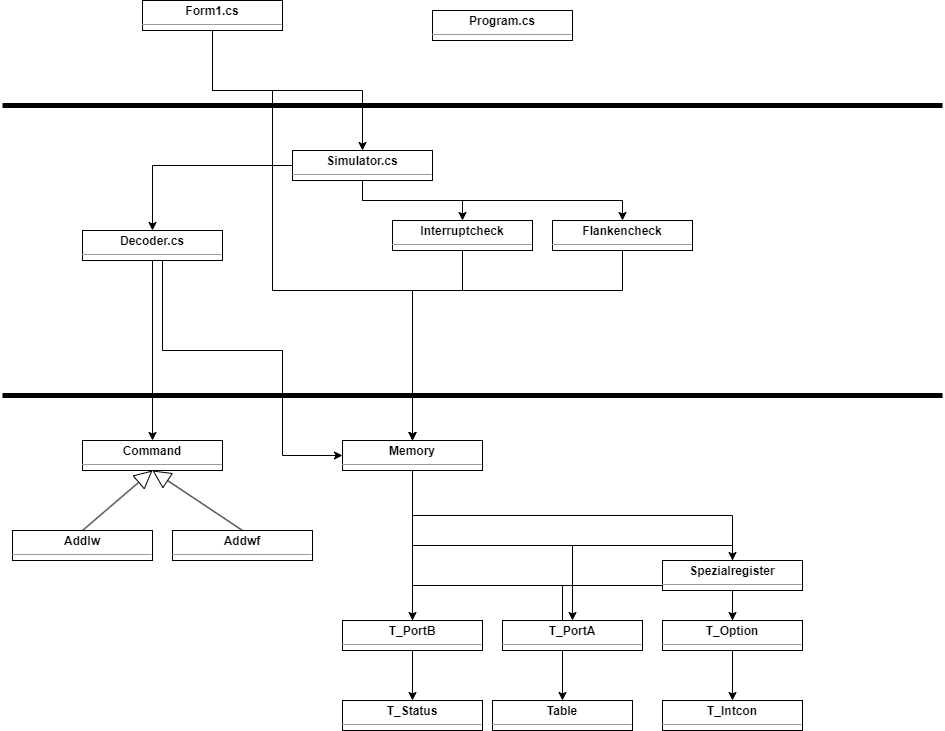
\includegraphics[width = \linewidth]{"images/classdiagramm.png"}
        \caption{Classendiagramm mit Unterteilung in Schichten}
    \end{figure}

    \section{Refactoring}\label{sec:refactoring}


    In diesem Abschnitt wird eine Auswahl der identifizierten Code Smells und eingesetzten Refactorings vorgestellt. Hierbei handelt es sich natürch nicht um alle Beispiele welche in diesem Projekt vorkommen und es sind noch einige, vor allem Code Smells, im Code vorhanden. 

    \subsection{Code Smells}

    \subsubsection{Switch Statement}

    Die urspüngliche 'Decode'- Klasse beinhaltet exakt eine Methode mit dem Namen 'analyse()', welche einen Operationcode einließt und den entsprechenden Command aufruft. In dieser sind eine Reihe von Code Smells zu erkennen: Unter Anderem Code Comments, was hier auf eine Long Method hindeutet.
    Kernproblem dieser Methode ist jedoch das sich darin befindende riesige Switch-Statement und damit der dazugehörige Code Smell. Dies erschwert es unter anderem, einen neuen Command dem PIC-Simulator hinzuzufügen,
    da dieser dem Switch-Statement hinzugefügt werden muss. Dieser Vorgang kann fehleranfällig sein und außerdem wird dadurch das Open-Closed-Principle der SOLID Principles(\autoref{subsec:solid}) verletzt. 
    Dieser Code Smell wurde durch den Einsatz einer Zuständigkeitskette als Entwurfsmuster behoben, welches in \autoref{sec:entwurfsmuster} erläutert wird.

    \subsubsection{Long Method}

    Eine Weitere Methode welche deutlich zu groß ist und definitiv unter den Code Smell Long Method fällt ist die ehemalige 'writeByte()' Methode der 'Memory'- Klasse. Diese ist schnell zu erkennen, da auch hier einige Code Comments zu finden sind und auch einfach an der unnötig hohen Zeilenanzahl.
    Eine zu lange Methode führt zu einer Reihe möglicher Probleme. Dazu gehören erschwerte Lesbarkeit und Wartung sowie erhöhtes Fehlerrisiko und Risiko auf unnötige Wiederholung von Code. Damit werden unter anderem die Programming Principles DRY und Single Responsibility verletzt. 
    Behoben wird der Code Smell durch ein Extract Method refactoring, welches unten beschrieben wird.
    
    \subsubsection{Duplicated Code}\label{subsubsec:duplicated_code}

    Die einzelnen Commands beinhalten zu einem größten Teil gleiche oder ähnliche Funktionen, welche in jedem einzelnen Command neu implementiert wurden. Dadurch war ein beträchtlicher Teil des Codes mehrfach vorhanden, was zur Folge hatte,
    dass eine Änderung immer an allen Commands durchgeführt werden musste. Dies wurde in dem Schritt gelöst, in dem auch die 'Cpu'- Klasse aufgelöst wurde und jeder Command in einer eigenen Klasse definiert wurde. 
    Dabei wurde eine abstrakte Oberklasse 'Command' eingeführt, in welcher die sich wiederholenden Funktionen definiert sind.

    \subsubsection{Large Class}
    Für den Code Smell Large Class gibt es zwei auffällige Beispiele. Bevor der Code Refactored wurde basierte der Großteil der Funktionalität auf zwei Klassen, 'Cpu' und 'Simulator', welche beide aus einigen hundert Zeilen Code bestanden und eine große Anzahl an Methoden beinhalteten.
    Dieser Aufbau verstößt gegen einige der Programming Principles, aber primär dem Single Responsibility Principle, weches in \autoref{subsubsec:single_responsibility} erläutert wird. Er stört dabei die Les- und Wartbarkeit des Codes sowie die Möglichkeit zur Erweiterung von Funktionalitäten.
    Aus diesem Grund wurde die 'Cpu'- Klasse komplett aufgelöst und die  Simulator Klasse mit Hilfe eines Extract Class Refactorings, welches anschließend erläutert wird, verkleinert.

    \subsection{Refactoring}
    \subsubsection{Extract Method}
	Um die Simulator Klasse zu vereinfachen wurden die Methoden welche die Register erstellen und Anfangs mit Daten füllen jeweils in eigene Klassen gepackt und in einem Namespace untergebracht.
	Hiermit ist die Simulator Klasse um einiges geschrumpft.
	Um noch ein wenig weiter für Ordnung zu sorgen ist eine Methode erstellt worden welche die Aufgebe hat aus den Register Klassen oObjekte zu erstellen und deren Methode zum füllen aufzurufen. 
	
    \subsubsection{Interupt- und Flanken-Check}
   	Auch die Methoden für die Checks auf Interrupts und Flanken wurden im Rahmen des Refactoring in eigene Klassen gepackt um die Simulator Klasse zu vereinfachen.
   
   
   	\section{Unit-Tests}
    Die Unit-Test können im Ordner /PicSimTest gefunden werden. 
	Mit diesen Tests werden viele unserer Klassen getestet.
	Um die (Unit-)Tests für C\# zu schreiben wird hier das MSTest Framework genutzt welches es in Kombination mit Visual Studio ermöglicht die Tests automatisch laufen zu lassen.

    \subsection{Einsatz von Mocks}
    Zum Testen einiger Methoden werden Mock-Objekte erstellt um die Test so abgetrennt wie möglich halten zu können.
	Um dies einfach machen zu können wird moq\footnote{\url{https://github.com/moq/moq4}} genutzt.
	Moq ermöglicht es einfach aus Klassen Mock-Objekte zu erstellen welche dann zum Testen genutzt werden können.
	
    \subsection{ATRIP-Regeln}
	\label{subsec:atrip-regeln}

    \subsubsection{Automatic}
	Visual Studio ermöglicht es mit einem Klick alle Test Durchlaufen zu lassen und findet hier auch neue Test im Projekt \verb|PicSimTest| wenn diese mit den richtigen Attributen \verb|[TestClass]| oder \verb|[TestMethode]| versehen wurden.
	
    \subsubsection{Thorough}\label{subsec:thorough}
    Da die Klassen der Befehle und der Register den Großteil der Rechenarbeit des simulierten Pic erledigen werden diese auf ihr verhalten getestet.
    

    \subsubsection{Repeatable}
    Da für unsere Tests die Daten Statisch sind und direkt in den Test Methoden eingebettet sind sollten die Tests jederzeit,  auch auf anderen Systemen, reproduzierbare Ergebnisse liefern.

    \subsubsection{Independent}
	Um Unabhängigkeit voneinander zu haben sind die Tests für eine Klasse jeweils in einer eigenen TestClass und darin sind nur die Testmethoden für die Methoden der zu Testenden Klasse enthalten.
 	Durch die Konzeption der Tests können diese in belibiger Reihenfolge oder auch einzeln Ausgeführt werden. 
 	Dies Ermöglicht es auch einzelne Programmabschnitte zu testen ohne auf viele Tests warten zu müssen.
    \subsubsection{Professional}
    Um die Absicht des Tests klar und und einfach verständlich zu gestalten sind die Testmethoden und Testklassen Namen selbsterklärend gewählt. 
    So heißt die Klasse des Test für den im Simulator genutzten Befehl \verb|Addlw|  \verb|AddlwTest|.
    Auch die Test Methoden selbsterklärend so wird die Methode \verb|isOpCode| im Objekt Addlw von der Methode \verb|isOpCode_rightCode| auf Verhalten bei Eingabe des richtigen Codes getestet.

    \section{Programming Principles}

    \subsection{SOLID}\label{subsec:solid}
    
    \subsubsection{Single responsibility principle}\label{subsubsec:single_responsibility}
    Das Single Responsibility Principle sagt aus, dass eine Klasse nur exakt für eine Funktionalität zuständig ist. Im Umkehrschluss bedeutet dies auch, dass es immer nur einen einzigen Grund geben soll, warum die Klasse geändert werden müsste.
    Ziel dieses Prinzips ist niedrige Kopplung sowie niedrige Komplexität innerhalb der Klasse. In diesem Projekt wurde dieses Prinzip in einigen Klassen angewandt. ein Beispiel dafür sind die Klassen der einzelnen Register. 
    Diese verfügen nur über eine einzige Zuständigkeit: das Auffüllen neuer Datentabellen zur dargestellung der einzelnen Register des Simulators.
    \\
    \begin{figure}
        \centering
        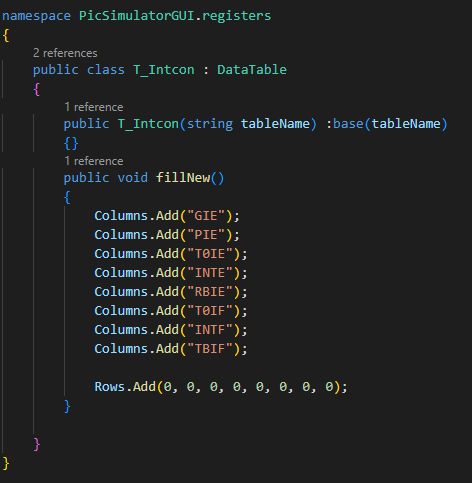
\includegraphics[width = .7 \linewidth]{"images/register.png"}
        \caption{T_Intcon Klasse}
    \end{figure}
    

    Ein Negativbeispiel ist vor allem die 'Forms'-Klasse, welche viele Funktionen durchführt und damit eine hohe anzahl an Zuständigkeiten und Änderungsdimensionen besitzt. Auch die 'Simulator'-Klasse fällt trotz der Refactorings immernoch in diese Kategorie. 



    \subsubsection{Open/Closed principle}
    Für gute Software ist es wichtig, dass sie offen für Erweiterung aber geschlossen für Veränderung ist. Code so zu gestalten, dass er überhaupt nicht verändert werden muss ist oft nicht möglich, es sollte aber so minimal wie möglich gehalten sein. Ein Beispiel im Code sind dabei die einzelnen Commands.
    Diese sind alle in einzelnen Klassen definiert, welche von einer abstrakten Oberklasse "Command" erben. Soll ein neuer Command hinzugefügt werden, so kann eine neue Unterklasse davon erstellt werden. Um diese im Projekt zu integrieren, muss dieser lediglich der 'CommandList' in der 'Decoder'- Klasse hinzugefügt werden.
    Diese minimale Modifikation des Codes wird durch den Einsatz eines Entwurfsmusters in \autoref{sec:entwurfsmuster} ermöglicht. 

    \begin{figure}
        \centering
        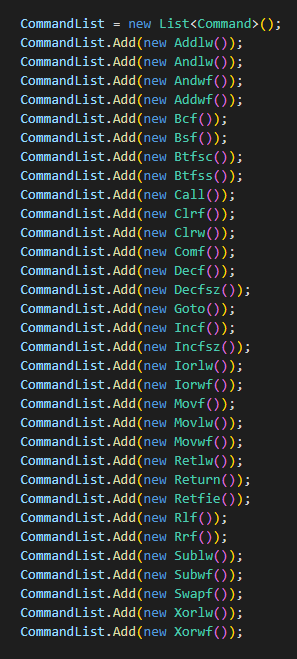
\includegraphics[width = .7 \linewidth]{"images/commandlist.png"}
        \caption{liste der einzelnen Commands}
    \end{figure}


    \subsection{GRASP}

    \subsubsection{High Cohesion}

    Kohäsion steht dafür, wie stark eine Klasse in sich zusammenhält, also wie stark die einzelnen Methoden und Attribute logisch miteinander zusammenhängen. In einer Klasse ist eine hohe Kohäsion erstrebenswert, da in diesem Fall nur die Methoden und Attribute in der Klasse vorhanden sind, die auch unbedingt benötigt werden.
    Eine hohe Kohäsion führt damit oft zu einer kleinen Klasse und führt meist automatisch zu einem Single Responsibility Principle. Ein Beispiel für eine Klasse mit einer hohen Kohäsion ist die 'Decoder'- Klasse, welche ausschließlich aus teilen besteht, welche für die Dekodierung von Operationcodes benötigt werden. 
    Eine Klasse mit einer extrem niedrigen Kohäsion ist die 'Forms'-Klasse. Sie enthält eine große Anzahl an Methoden, deren Aufgaben logisch nichts miteinender zu tun haben.  

    \subsubsection{Low Coupling}
    
    Kopplung ist die Abhängigkeit einer Klasse von seinem Umfeld. Die am leichtesten zu erkennenden Abhängigkeiten sich dabei die von anderen Klassen. Eine niedrige Kopplung ist sinnvoll, da dies zu einer erhöhten Flexibilität der führt. Solche Klassen sind leichter Wiederverwendbar, leichter lesbar und deutlich besser wartbar, da weniger Rücksicht auf die Abhängigkeiten genommen werden muss. 

    
    \subsection{DRY -- Don't Repeat Yourself}
    Das DRY Principle ist eng mit dem Code Smell Duplicated Code verbunden, also mit Codeabschnitten, welche mehrfach im COde vorkommen. Um diese zu vermeiden besagt DRY, dass es für jede Information nur eine einzige Quelle gibt, auf welche der rest des Codes zugreift.
    Aufgrund der Ähnlichkeit mit Duplicated Code ist das beste Beispiel für den Einsatz des DRY Principles die auslagerung von Methode wie 'carryCheck()', 'zeroFlagCheck()' oder 'writeToDestination()' von den einzelnen Commands in eine abstrakte Oberklasse. So müssen diese nicht in jeder konkreten Klasse neu definiert werden. Für ein genaueres Bespiel, siehe \autoref{subsubsec:duplicated_code}.  

    \begin{figure}
        \centering
        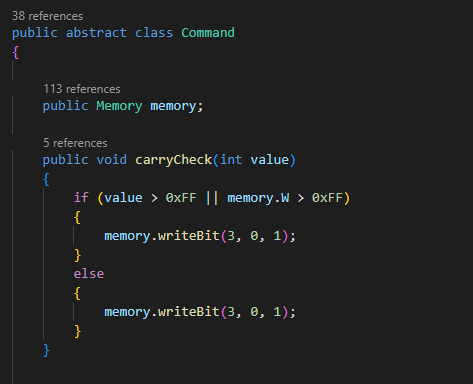
\includegraphics[width = .7 \linewidth]{"images/abstractCommand.png"}
        \caption{Abstrakte Command Klasse mit ausgelagerter Methode}
    \end{figure}

    \section{Entwurfsmuster: Zuständigkeitskette}\label{sec:entwurfsmuster}

    Wie bereits in den Code Smells in \autoref{sec:refactoring} erwähnt, handelte es sich bei dem Teil des Codes, welcher die Operationcodes des eingelesenen Programmes decodiert um ein überdimensionalen Switch- Statement.
    Dieser sollte vermieden werden. Außerdem sollte die 'Cpu'- Klasse aufgelöst werden und jeder Command als eigene Klasse dargestellt werden. Zur Lösung dieser Probleme wurde die Zuständigkeitskette entdeckt.
    Dabei handelt es sich um ein Entwurfsmuster aus der Reihe der Verhaltensmuster, zu welchen auch der Beobachter gehört. 
    \\
    Eine Zuständigkeitskette dient dazu, verschiedene Anfragen eines Clients zu bearbeiten, welche an das selbe Interface gesendet werden. Dieses Interface wird dabei als Base Handler bezeichnet. Dazu wird die Anfrage an eine Kette von sogenannten konkreten Handlern geleitet.
    Ist eine Handler für die jeweilige Anfrage zuständig, so wird sie von diesem bearbeitet. Wenn nicht, wird sie an den nächsten Handler der Kette weitergegeben. Der Client muss dabei nicht wissen, von welchem Handler die Anfrage bearbeitet wurde und die konkreten Handler kennen lediglich ihren jeweilige Nachfolger.
    \\
    In diesem Fall ist die Anfrage der Operationcode des aktuellen Befehls im eingelesenen Programm, welcher von der 'Simulator'- Klasse in der Rolle als Client gestellt wird. Die konkreten Handler sind die einzelnen Commands, welche in der Methode 'isOpCode()' überprüfen, ob sie für den Befehl zuständig sind.
    Im gegensatz zur Originalimplementierung ist hier allerdings die 'Decoder'- Klasse zwischen Client und konreten Handlern, in welcher alle Handler in einer Liste aufgeführt sind, durch welche dann iteriert wird. Anstatt dass jeder konkrete Handler seinen Nachfolger und nur diesen kennt, wird die Kette vollständig in der 'Decoder'- Klasse definiert.
    Diese Praxis weicht zwar von dem origalen Entwurfsmuster ab, verringert aber die Anzahl der Methoden in der 'Command'-Klasse und gestaltet den Aufbau und damit auch die Erweiterung der Kette übersichtlicher, da neue Commands lediglich der 'CommandList' hinzugefügt werden müssen,
    anstatt sie einzeln zu instanziieren und sie als nächsten Handler des zuvor letzten zu definieren.

    \begin{figure}
        \centering
        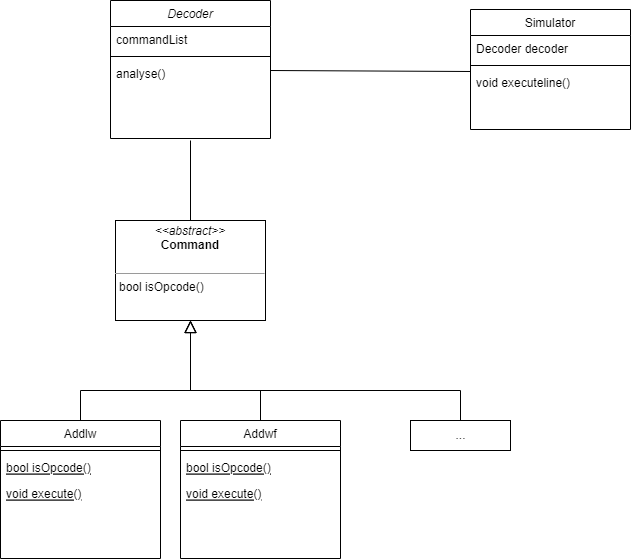
\includegraphics[width = .7 \linewidth]{"images/zustaendigkeitskette.png"}
        \caption{Zuständigkeitskette in UML}
    \end{figure}

\end{document}
